\paragraph{ECIES Encryption Implementation}

--- description of classes used ---

--- update the figure below, adding packages to it ---

\begin{figure}[ht!]
	\centering
	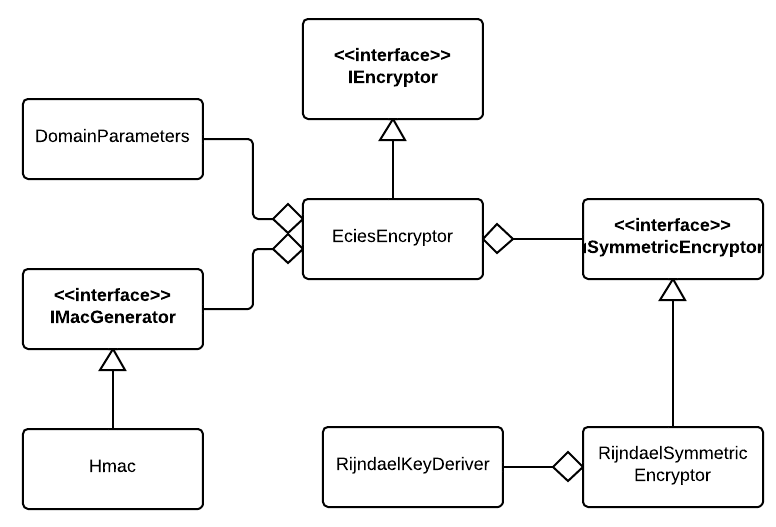
\includegraphics[width=90mm]{img/naive_implementation__encryption__ecies_class_diagram.png}
	\caption{Class Diagram of structure around the ECIES encryption implementation}
	\label{ecies_class_diagram}
\end{figure}

This adds new dependencies to the project: AES and HMAC.

C\# has built-in support for Rijndael\footnote{http://msdn.microsoft.com/en-us/library/system.security.cryptography.rijndaelmanaged.aspx}
(AES)\footnote{See also: http://msdn.microsoft.com/en-us/magazine/cc164055.aspx}, and trusting this implementation is assumed safe for
the scope of this project. Again, the importance of the naive implementation is to show a full, working stack with naive implementations
of the basics of Elliptic Curves (but not other basic constructs).

It is possible to set a specific key in \verb+RijndaelManaged+, so what is now needed is the key derivation function, which will have to
be constructed for the purpose.

--- key deriv func ---

HMAC is supported in C\# as well\footnote{http://msdn.microsoft.com/en-us/library/system.security.cryptography.hmac.aspx; example: http://social.msdn.microsoft.com/Forums/vstudio/en-US/c963042a-24d3-45bb-ad00-272c00ed0bd4/encryptdecrypt-using-hmac-algorithm-in-c?forum=csharpgeneral}.

--- actual encryption ---